\subsection{Blockchain}

Para el ecosistema de blockchain se decidió utilizar la red de Ethereum \cite{wood2014ethereum}, al ser una blockchain popular y muy utilizada para el desarrollo de aplicaciones descentralizadas nos permite demostrar y comparar los casos de uso contra nuestra solución en IPFS.

\subsubsection{Swarm}

Existen varias soluciones de almacenamiento descentralizado dentro del ecosistema blockchain, en este caso, para el desarrollo del sitio web estático optamos por Swarm al estar basado en una \textit{sidechain} de Ethereum.

\paragraph{Feed} El contenido que se publica en Swarm tiene asociado un CID, esto lo hace inmutable. Para permitir cambios manteniendo la inmutabilidad del contenido en Swarm existen los \textit{feeds} que funcionan de manera similar a los IPNS de IPFS. Es un puntero, con CID fijo, a un archivo. Esto permite actualizar el archivo al que apunta un \textit{feed} manteniendo un punto de entrada fijo al sitio web.

\paragraph{Postage stamps} Esta es la forma de pagar por el uso del almacenamiento en la red de Swarm. Posee un \textit{time-to-live} (TTL) que es calculado en base a los valores de \textit{depth} y \textit{amount} indicados al momento de la creación del \textit{stamp} \cite{swarm-postage-stamps}.

\paragraph{Despliegue} Para el despliegue del front-end es necesario primero comprar un \textit{postage stamp} con la moneda BZZ y luego con la herramienta \texttt{swarm-cli} \cite{swarm-cli} se publica el sitio web indicando el \textit{feed} correspondiente. Durante el desarrollo encontramos que no existe un \textit{gateway} público que apunte a la testnet de Sepolia y nos permita probar el despliegue sin necesidad de utilizar dinero real. Es por esto que se levantó un nodo de Swarm configurado para que apunte a la testnet de Sepolia y un \textit{gateway} que utilice este nodo mediante la herramienta \texttt{gateway-proxy} \cite{gateway-proxy} que provee el equipo de Swarm.

\subsubsection{Ethereum}

Para los casos de uso del repositorio de conocimiento y el mensajero en tiempo real necesitamos una herramienta que funcione de manera \textit{read-write} y como Swarm solamente se encarga de archivos estáticos buscamos alguna alternativa dentro del ecosistema blockchain. Para esto terminamos usando Ethereum.

\begin{figure}[H]
    \centering
    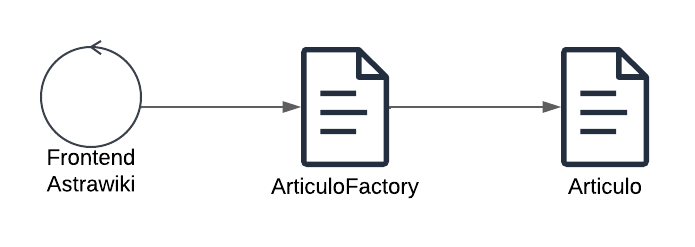
\includegraphics[width=0.5\linewidth]{img/astrawiki-articulo-factory.png}
    \caption{\textit{Smart contracts} que intervienen en el repositorio de conocimiento}
    \label{fig:aw-eth-articulo-factory}
\end{figure}

Ambos casos de uso resultaron muy similares en su resolución, haciendo uso del patrón de diseño \textit{Factory}. Existe un smart contract Factory que crea otros smart contracts (Artículo o Chat, según el caso de uso).

\begin{figure}[H]
    \centering
    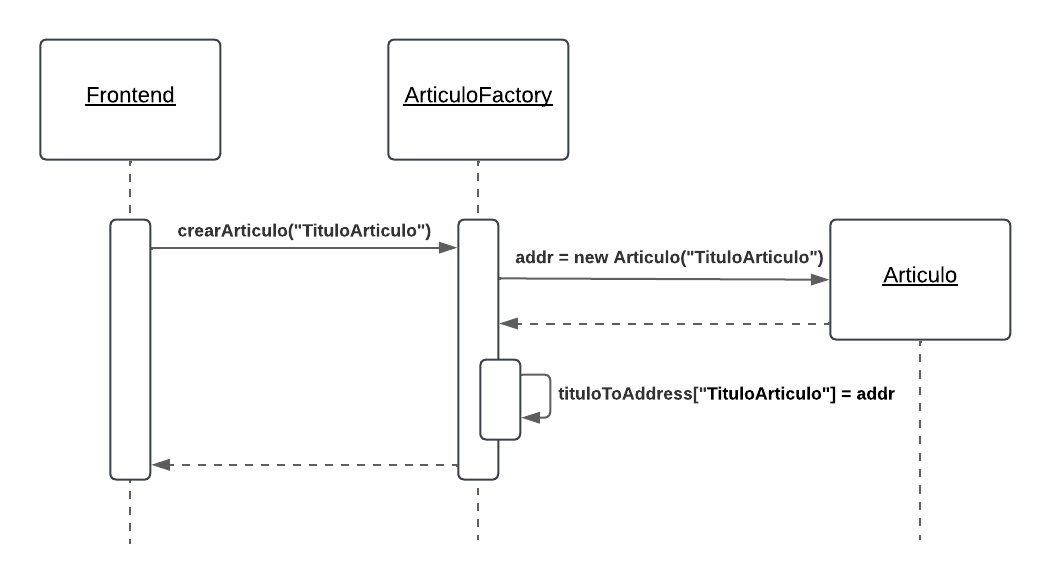
\includegraphics[width=0.75\linewidth]{img/ds-aw-eth-crear-articulo.png}
    \caption{Creación de un artículo}
    \label{fig:ds-aw-eth-crear-articulo}
\end{figure}

De esta manera el \textit{Factory} tiene un \textit{mapping} con todos los artículos creados y las direcciones correspondientes para accederlos. Si se quisiera acceder a un Artículo en particular primero se tiene que consultar al \textit{Factory} para obtener la dirección del mismo y, como cada artículo es un \textit{smart contract} en sí mismo, se puede consultar o modificar su contenido directamente interactuando con el Artículo en particular como se puede ver en la Figura \ref{fig:ds-aw-eth-obtener-contenido-articulo}.

\begin{figure}[H]
    \centering
    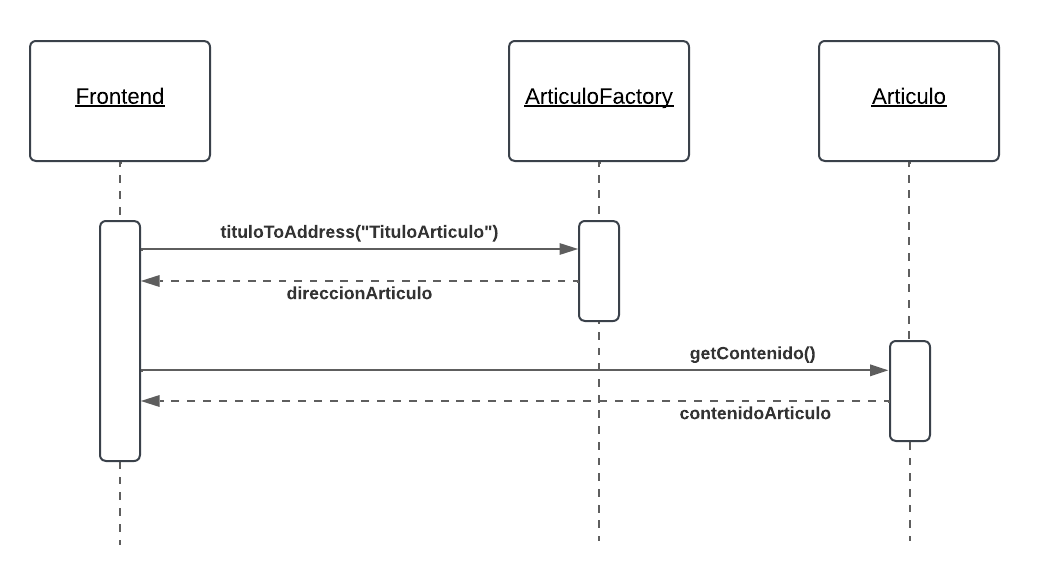
\includegraphics[width=0.75\linewidth]{img/ds-aw-eth-obtener-contenido-articulo.png}
    \caption{Obtención del contenido de un artículo}
    \label{fig:ds-aw-eth-obtener-contenido-articulo}
\end{figure}

La principal diferencia entre el repositorio de conocimiento y el mensajero en tiempo real está en que los mensajes del mensajero tienen que ser vistos por los demás usuarios que participan de la conversación en el momento que se envían. Esto no es estrictamente necesario en el repositorio de conocimiento pero sí lo es en el mensajero.

Para afrontar este requisito se utilizaron los eventos de Solidity (el lenguaje de programación en el que se desarrollan los \textit{smart contract} de Ethereum). Funciona de la siguiente manera, al momento de enviar un mensaje se emite un evento. Este evento se recibe en un listener que fue previamente inicializado al instante previo de haber obtenido el Chat en el frontend. Al recibir este evento el frontend puede actualizar la pantalla mostrando el mensaje nuevo sin necesidad de obtener todos los mensajes.

% TODO: insertar gráfico del flujo de un evento al enviar un mensaje 

Por otro lado, para el mensajero en tiempo real necesitamos una manera de identificar a cada usuario. Para esto se hizo uso de las \textit{wallets}. Cada usuario se identifica utilizando su \textit{wallet}, que tiene una clave pública, que pasa a ser el identificador del usuario, y una clave privada la cuál es necesaria para firmar transacciones en nombre del usuario, que en nuestro caso funciona a modo de contraseña. Además, para que la lectura de las conversaciones sean más usables, se agregó la posibilidad de generar un nombre de usuario asociado al identificador del mismo. A este nombre de usuario lo llamamos alias y es único para todos los Chats asociados a un mismo ChatFactory. Una vez el usuario se conecta con su \textit{wallet}, puede elegir un alias y cambiarlo cuando desee siempre y cuando no exista actualmente algún otro usuario con ese mismo alias.

Finalmente, nos queda la funcionalidad de que un usuario pueda responder a otro mensaje. Primero necesitamos una manera de identificar a cada mensaje de manera unívoca. El identificador de cada mensaje se genera hasheando el timestamp del bloque, el identificador del emisor y la cantidad de mensajes en el chat en el momento que se envía. Luego, cuando se responde a otro mensaje se almacena el identificador del mensaje al que se está respondiendo (el mensaje padre) dentro de la estructura del mensaje que se está enviando. Todo esto se resuelve dentro del \textit{smart contract} del Chat correspondiente.
